\documentclass[12pt, a4paper]{article}

%Paketler ve kullaımları
\usepackage[ddmmyyyy]{datetime}
\usepackage{graphicx}
\usepackage{ragged2e}
\usepackage{float}



%overrides
\renewcommand{\dateseparator}{.}
\renewcommand{\figurename}{Şekil}
\renewcommand{\refname}{Kaynaça}
\restylefloat{figure}

%ayarlamalar
\title{Gaussian Splatting Yöntemi ve Yapay Zeka Yardımı ile 3D Model Oluşturulması}
\author{Mert Seyit Yılmaz}
\date{09.03.2024}
\graphicspath{ {./images} }
\floatstyle{boxed} 



\begin{document}
	
	\begin{figure}
		\centering
		
\includegraphics{ksbu.png}
	\end{figure}
	
	\maketitle
	
	
	\section{Giriş}
	
	Günümüzde teknolojinin ilerlemesi ile birlikte 3 boyutluluk önemli yol kat etmiş durumdadır. Oyunlar, Virtual Reality (VR, Sanal Gerçeklik), Metaverse, Sanal Avatar gibi kavramlarda artık 3 boyutlu ortamlar oluşturularak insanlara gerçek dünyanın sanal kopyaları oluşturulmaya çalışılıyor. 3 boyutlulukta en önemli nokta, nesnelerin ve ortamların 3 boyutlu birer kopyasını oluşturmaktır. Bu işi gerçekleştirebilmek için Blender, SketchUp, AutoCAD, Tinkercad (CAD: Computer Aided Design, Bilgisayar Destekli Tasarım), Cinema 4D gibi uygulamar kullanılır. Bu uygulamalar sizin 3 boyutlu dünyanızı ve içerisindeki nesneleri modellemenizi sağlar.
	
	\bigskip
	
	3D nesne tasarımı gerek uygulamaların öğrenim zorluğu, gerek tasarım sürecinden dolayı epey zaman alan bir süreçtir. Bu proje Gaussian Splatting yöntemi ve Yapay Zeka yardımı ile nesnelerin ve ortamların 3D modellerinin çıkartılması ve kullanıma hazırlamayı hedeflemektedir. 
	
	
	
	\section{Literatür Araştırması}
	
	Gaussian Splatting kavramındaki Gaussian 1800'lerde Ayrık Olasılık Dağılımı Teknikleri üzerine çalışmalar gerçekleştirmiş Carl Friedrich Gauss'un soy adından, Splatting ise bir kar topunun bir duvara çarparken çıkardığı sesten gelmektedir. Gaussian Splatting temel 3D oluştuma uygulamarında iyi tanımlanmış üçgenler ve yüksek çözünürlüklü pikseller yerine bulanık bulutlar kullanarak içeriği temsil etmeye çalışır. \cite{what-is-gaussian-splatting}
	
	\bigskip
	\begin{figure}[h]
		
		\centering
		\includegraphics{images/gausiano.png}
		\label{Gaussian Splatting}
		\caption{Gaussian Splatting'in Çalışma Mantığı}
	\end{figure}
	
	\bigskip
	
	Gaussian Splatting kavramı ilk olarak Ağustos 2023'de ortaya çıktı ve çıktığı günden bu yana büyük bir ses getirdi. Gaussian Splatting nesnelerin her açıdan çekilmiş fotoğrafları veya videoları üzerinden nesnenin 3D bir görüntüsünü sağlar. Buradan üretilen çıktı henüz 3D ortamlarda kullanıma uygun değildir. Çünkü oluşturulan 3D görüntünün bir .obj uzantılı dosya veya mesh adı verilen bir formatta olması gerekmektedir.
	
	\bigskip
	
	Şu anda Gaussian Splatting'in yaptığı gibi video veya fotoğraf üzerinden 3D modeller oluşturmaya yönelik yöntem ve teknolojiler bulunmaktadır.
	Bunlardan en bilineni Neural radiance field (NeRF) yöntemidir. NeRF, seyrek iki boyutlu görüntülerden bir sahnenin üç boyutlu temsilini yeniden oluşturmak için derin öğrenmeye dayalı bir yöntemdir. NeRF, tüm nesneyi veya sahneyi yapay bir sinir ağına kodlamayı içerir; bu ağ, farklı açılardan yeni 3B görünümler oluşturmak için 2B görüntünün herhangi bir noktasındaki ışık yoğunluğunu - veya parlaklığı - tahmin eder  \cite{NeRF} \cite{what-is-nerf}
	
	
	
	\bigskip
	\begin{figure}[h]	
		\centering
		\includegraphics[width=1\textwidth]{images/nerf-and-gaussian-splatting.png}
		\label{Differences between Gaussian Splatting and NeRF}
		\caption{3D Modellemede kullanılan NeRF ve 3D Gaussian Splatting'İn çalışma mantığı.}
	\end{figure}
	
	\begin{figure}[!h]	
		\centering
		\includegraphics[width=1\textwidth]{images/polycam-gaussian-splatting-and-nerf-capture.jpg}
		\label{Gaussian Splatting and NeRF examples}
		\caption{polycam web sitesi üzerinden üretilen örnek bazı 3D model uygulamaları. Soldaki görsel arka planda NeRF sistemi kullanılarak oluşturulmış bir model. Sağdaki görsel gaussian splatting kullanılarak oluşturulmuş bir model. Daha fazla örnek için www.poly.cam ' ı ziyaret edebilirsiniz. \cite{polycam-exp}}
	\end{figure}
	
	
	\section{Metodoloji}
	
	Projedeki amaç, Gaussian Splatting ile üretilen 3D mekanların, modellerin ve sahnelerin 3D yapılarını oluşturmak ve yardımcı programlar (CloudCompare, SuperSplat, Blender, Unity, Unreal Engine) ve Yapay Zeka Algoritmaları kullaılarak görüntülerde oluşan kirliliklerin (unnecessery point clouds) temizlenmesi olacaktır. Bu temizlemelerin yapılması önce uygulama ortamlarında yapılacaktır. Daha sonra temizleme işlemleri yapay zeka tarafına aktarılacaktır.
	
	\bigskip
	
	Çıktı verilerinin temizlenmesi aşamasında kullanmak istediğimiz birincil uygulama Blender uygulaması olacaktır. Blender, geniş çapta kullanılan bir 3D modelleme uygulamasıdır. İçerisine kurabileceğimiz eklentiler (add-on) sayesinde Gaussian Splatting uzantılı (.splat) çıktı verilerinin işlenmesi amaçlanmaktadır.
	
	\bigskip
	
	Çıktı verilerinin kullanılabilir hale getirilmesi hedeflenmektedir. Bu amaçla da CloudCompare uygulaması kullanılacaktır. Bu uygulama, point cloud verisinden mesh dosyası üretmeye yardımcı olacak özellikler barındırşmaktadır. Üretmiş olduğumuz temizlenmiş Gaussian Splatting çıktılarını daha sonra bu uygulama üzerinden işlemeyi amaçlamaktayız.
	
	\bigskip
	
	Son olarak üretimiş olduğumuz mesh verilerinin 3D ortamlarda kullanılması amaçlanmaktadır. Bu çıktıların kullanım alanları oldukça geniştir. Hedef doğrultusunda Unity, Unreal Engine gibi oyun motorları üzerinde çıktı verilerinin testi gerçekleşecektir.
	
	
	
	
	
	
	%Kaynakçayı
	\bibliographystyle{ieeetr}
	\bibliography{references.bib} 
	
	\section{İş Planı}
	\begin{figure}[h]	
		\centering
		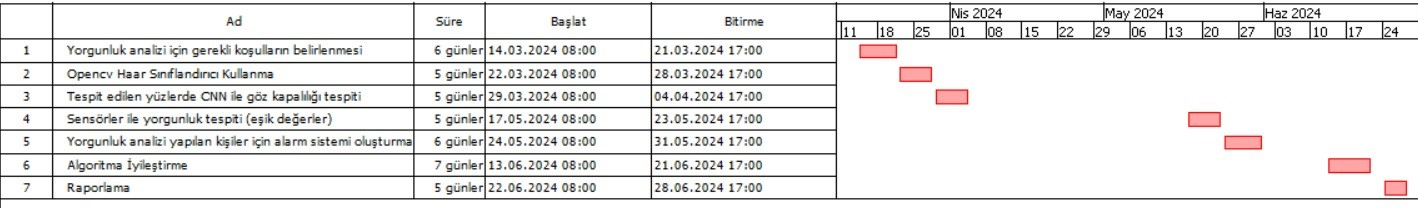
\includegraphics[angle=90, height=\textheight, ]{images/gantt.jpg}
		\label{Gantt Chart}
		\caption{Gantt Şeması}
	\end{figure}

	

\end{document}